\section{Computational complexity}
Let us define some notation.
\begin{defn}[Big $\mathcal{O}$ notation]
   Let $f$ be a real or complex valued function and $g$ a real valued function. Let both functions be defined on some unbounded subset of positive real numbers. One writes
   \begin{equation*}
       f(x) = \mathcal{O}(g(x)) \quad \text{as} \quad x \rightarrow a
   \end{equation*}
   if 
   \begin{equation*}
      \lim_{x \to a} \sup{\frac{\abs{f(x)}}{g(x)}} < \infty.
   \end{equation*}
   \end{defn}
   \begin{defn}[Big $\Omega$ Knuth notation]
      Let $f$ be a real or complex valued function and $g$ a real valued function. Let both functions be defined on some unbounded subset of positive real numbers. One writes
   \begin{equation*}
       f(x) = \Omega(g(x))
    \Longleftrightarrow
      g(x) = \mathcal{O}(f(x)).
   \end{equation*}
   \end{defn}
   
We take for granted some basic definitions of classical computational complexity theory and we proceed defying
\begin{defn}
\textbf{BPP} is the class of languages that can be solved in polynomial time by probabilistic Turing machines with error probability bounded by $1/3$. Using standard boosting techniques the error probability can then be made exponentially small in $k$ by iterating the algorithm $k$ times.
\end{defn}
\begin{defn}
\textbf{PSPACE} is the class of languages that may be solved on a Turing machine using a polynomial number of working bits, with no limitations on the amount of time that may be used by the machine.
\end{defn}
\begin{defn}
\textbf{BPQ} is the class of languages that can be solved in polynomial time by quantum Turing machines with error probability bounded by $1/3$. The error probability can be made exponentially small as in \textbf{BPP}.
\end{defn}
There are some evidence~\cite{Bennett_1997} that $\textbf{BQP} \neq \textbf{BPP}$ (i.e. polynomial-time quantum Turing machines are more powerful than polynomial-time probabilistic Turing machines). Since \textbf{BPP} is regarded as the class of all efficiently computable languages, this provides evidence that quantum computers could be inherently more powerful than classical computers in a model-independent way.

However exactly where \textbf{BQP} fits with respect to \textbf{P}, \textbf{NP} and \textbf{PSPACE} is as yet unknown. What is known is that quantum computers can solve all the problems in \textbf{P} efficiently and that there are no problems outside of \textbf{PSPACE} which they can solve efficiently. Therefore, \textbf{BQP} lies somewhere between \textbf{P} and \textbf{PSPACE}.
It has been demonstrated that
\begin{equation*}
   \textbf{P}   \subseteq \textbf{BPP} \subseteq \textbf{BQP}  \subseteq \textbf{PSPACE}
\end{equation*}
and so proving that $\textbf{BPP} \subset \textbf{BQP}$ would definitively establish that $\textbf{P} \subset \textbf{PSPACE}$, solving a major outstanding problem in computer science.
\begin{figure}[htb]
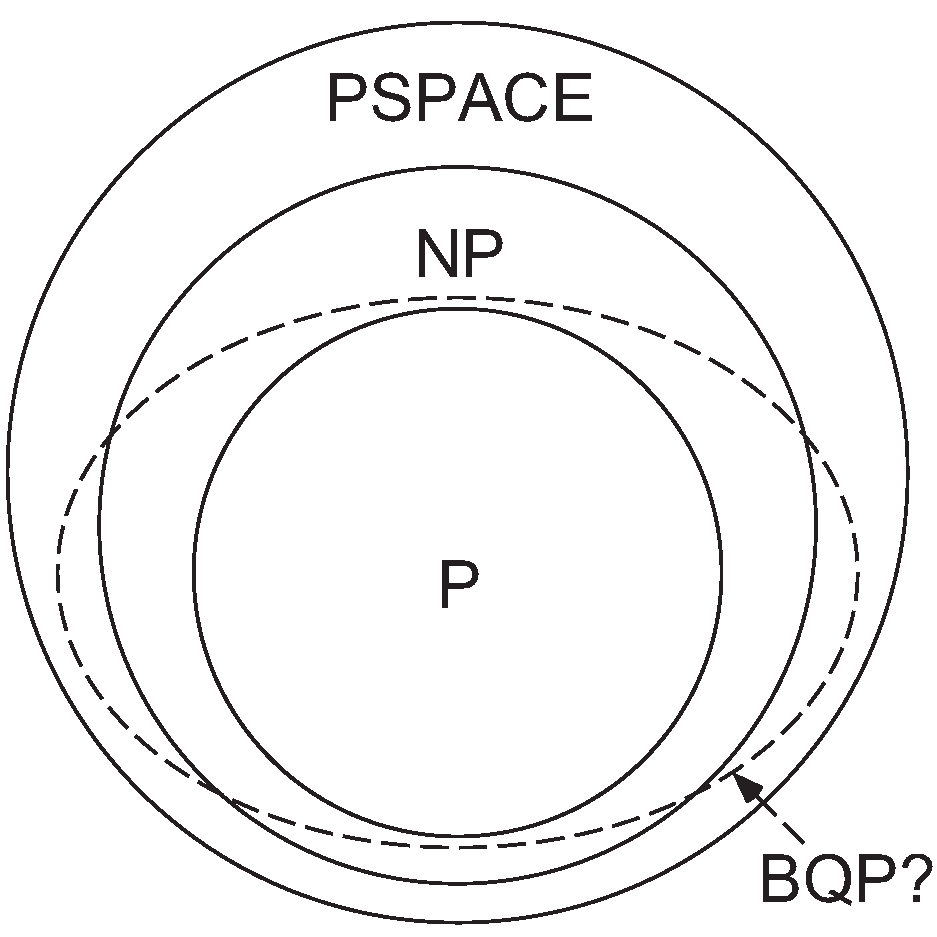
\includegraphics{computational-complexity.png}
\centering
\caption{The relationship between classical and quantum complexity classes.}
\end{figure}

Another open computational problem is $\textbf{NP} \stackrel{?}{\subseteq} \textbf{BQP}$.
We know that we can adopt a quantum search algorithm to solve any \textbf{NP}-complete\footnote{We can demonstrate that solving \textbf{NP}-complete problems in polynomial times would mean solving every other \textbf{NP} problem in polynomial time.} problem.


We can demonstrate that, because we know that the quantum search algorithm is optimal, this means that it is not possible to search an $N$ item search space in $\mathcal{O}(\log_2{N})$. If such an algorithm had existed, it would have allowed us to solve \textbf{NP}-complete problems efficiently on a quantum computer by transforming problems in \textbf{NP} into search problems.
This strongly suggests that \textbf{NP} is not included in \textbf{BQP}.

This does not rule out the possibility that \textbf{NP} $\subset$ \textbf{BQP}. What this result do establish is that there is no search-based method for attacking \textbf{NP}-complete problems.
However we note that it is widely believed that the search space of \textbf{NP}-complete problems has no structure and that the best possible method for solving such problems is to adopt an unstructured search method. Furthermore for many problems in the \textbf{NP}-complete class there is no better method known than exhaustive search of all the possible solution. If one takes this point of view this indicates that \textbf{BQP} does not contain \textbf{NP}-complete problems.
